% Provenance (never printed): see sources/outline_sources.md (Year 3: gravitational
% potential, spherical harmonics, J2, reference ellipsoid, geoid, satellite gravimetry,
% flexure of the lithosphere). Brief: sources/book5/BRIEFS.md, ch. 3. Curves from
% figdata/bachelor-3/hydrostatic_figure.py, ice_mass.py (IMBIE 2021), flexure.py.
% Exercise and problem values in the Book 5 scratch calculator calc/ch03.py.
\chapter{Gravitasi dan Bentuk Bumi}\label{ch:b3:gravity-geodesy}

Dua satelit terbang beriringan mengelilingi Bumi, pada ketinggian lebih dari
\qty{500}{km} dan berjarak sekitar \qty{220}{km} satu sama lain, dan mengukur jarak
antara keduanya setiap saat, dengan ketelitian hingga satu mikrometer.
% ledger: geod5:grace, geod5:grace-ranging
Ketika keduanya melintas di atas tempat yang massanya terkumpul, satelit di depan
lebih dulu tertarik maju dan jaraknya melebar; lalu satelit di belakang
tertarik dan jaraknya kembali menyempit. Dari perubahan kecil itu, bulan demi bulan sejak 2002,
medan gravitasi Bumi telah dipetakan seiring perubahannya: air yang tersimpan di
cekungan sungai naik dan turun mengikuti musim, dan lembaran es besar di
Greenland dan Antarktika kehilangan massa tahun demi tahun. Gravitasi menimbang
apa yang tak kasat mata. Bab ini membangun medan gravitasi planet berotasi dari
potensialnya, menemukan di dalamnya penggepengan dan momen inersia, lalu menelusuri
anomalinya hingga ke orbit, kemudian beralih ke salah satu hal yang diungkap gravitasi
di permukaan: \omterm{def:b3:gravity-geodesy:flexure}{lenturan litosfer} akibat beban sebuah gunung api.

\begin{recall}
Hukum gravitasi Newton, energi potensial gravitasi, dan
gaya sentrifugal dalam kerangka berotasi dibahas di buku fisika; momen inersia
benda tegar dan polinomial Legendre $P_2(x) = (3x^2 - 1)/2$ ada dalam
volume perguruan tinggi buku fisika dan buku matematika, modulus Young $E$ dan
rasio Poisson $\nu$ dalam volume Tahun 3 buku fisika. Geodesi dan
penggepengan $f = (a - b)/a$ elipsoid dengan semi-sumbu $a > b$ telah dijumpai di
kelas 10. Isostasi, kompensasi Airy, gravitasi normal, geoid, tinggi geoid,
dan anomali gravitasi telah didefinisikan dalam volume Tahun 1, pada bab
tentang isostasi dan anomali gravitasi.
\end{recall}

\section{Geopotensial}

Pada planet yang berotasi, benda yang diam merasakan tarikan massa planet
dan, dalam kerangka yang ikut berputar, gaya sentrifugal. Keduanya diturunkan dari
sebuah potensial.

\begin{definition}[Geopotensial]\label{def:b3:gravity-geodesy:geopotential}
Yang disebut \emph{geopotensial}\index{geopotensial} adalah energi potensial per satuan
massa, dalam kerangka yang berotasi bersama Bumi dengan kecepatan sudut $\omega$, dari
gravitasi dan gaya sentrifugal bersama-sama:
\[
  W(\mathbf r) = V(\mathbf r) + \Phi(\mathbf r),\qquad
  V(\mathbf r) = -G\int_{\text{Bumi}}\frac{\mathrm dm'}{|\mathbf r - \mathbf r'|},\qquad
  \Phi(\mathbf r) = -\tfrac12\omega^2 s^2,
\]
Di sini $s$ adalah jarak dari sumbu rotasi. Gravitasi
$\mathbf g = -\nabla W$, dan permukaan $W = \text{konstan}$ adalah
permukaan ekipotensialnya: gravitasi selalu tegak lurus terhadapnya.
\end{definition}

Tali unting menggantung searah $-\nabla W$, dan air diam mengendap pada
permukaan ekipotensial. Planet fluida yang berotasi karena itu mengambil bentuk salah satu
permukaan ekipotensialnya sendiri: potensial sentrifugal, yang paling dalam di khatulistiwa, menggelembungkan
bagian khatulistiwa dan menggepengkan kutub.

\begin{omfigure}
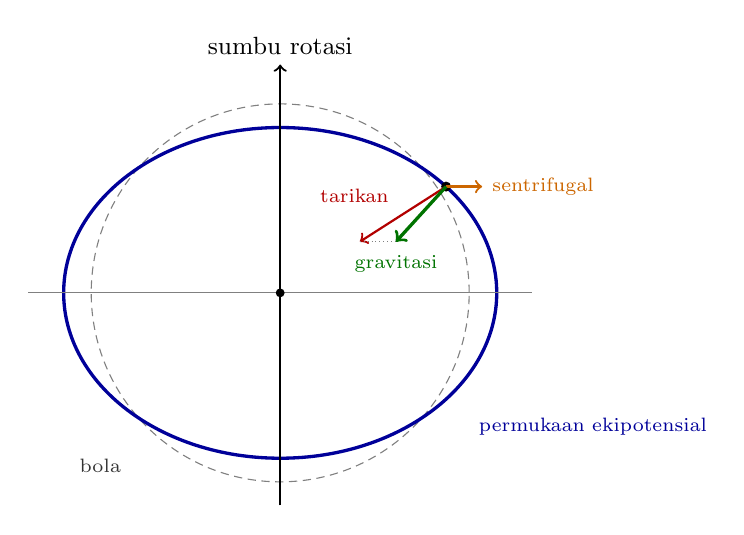
\begin{tikzpicture}[font=\small, x=1cm, y=1cm]
\draw[gray, densely dashed] (0,0) circle (2.4);
\draw[very thick, blue!60!black] (0,0) ellipse (2.75 and 2.1);
\draw[->, thick] (0,-2.7) -- (0,2.9) node[above] {sumbu rotasi};
\draw[gray] (-3.2,0) -- (3.2,0);
\fill (0,0) circle (1.6pt);
% a point at latitude 40 deg (parameter) on the ellipse; the attraction points at
% the centre, the centrifugal force is horizontal, and their sum is drawn along the
% inward normal of the ellipse: lengths solved so that the sum is normal (calc/ch03_fig.py)
\coordinate (P) at (2.107,1.350);
\fill (P) circle (1.8pt);
\draw[->, thick, red!70!black] (P) -- (1.012,0.650);
\node[font=\scriptsize, red!70!black, anchor=south east] at (1.50,1.02) {tarikan};
\draw[->, thick, orange!80!black] (P) -- (2.565,1.350) node[right, font=\scriptsize] {sentrifugal};
\draw[gray, densely dotted] (1.012,0.650) -- (1.470,0.650);
\draw[->, very thick, green!45!black] (P) -- (1.470,0.650);
\node[font=\scriptsize, green!45!black, anchor=north] at (1.470,0.600) {gravitasi};
\node[blue!60!black, anchor=west, font=\scriptsize] at (2.4,-1.7) {permukaan ekipotensial};
\node[gray!40!black, anchor=east, font=\scriptsize] at (-1.9,-2.2) {bola};
\end{tikzpicture}

\par\smallskip{\small Permukaan ekipotensial planet yang berotasi (skematis, penggepengan
sangat dibesar-besarkan). Pada setiap titik, gravitasi, yakni jumlah dari
tarikan dan gaya sentrifugal, tegak lurus terhadap permukaan ekipotensial; ia
tidak mengarah ke pusat, kecuali di kutub dan di khatulistiwa.}
\label{fig:b3:gravity-geodesy:equipotential}
\end{omfigure}

Di luar planet, potensial gravitasi memenuhi persamaan Laplace, dan
solusinya yang reguler di takhingga adalah harmonik bola pejal.

\begin{proposition}[Ekspansi harmonik bola dari geopotensial]\label{prop:b3:gravity-geodesy:harmonics}
Di luar benda bermassa $M$ dengan jari-jari khatulistiwa $a$, dengan titik asal di
pusat massanya dan sumbu $z$ searah sumbu rotasinya, potensial gravitasi
pada jarak $r$, kolatitud $\theta$, dan bujur $\lambda$ adalah
\begin{multline*}
  V = -\frac{GM}{r}\Biggl[1 - \sum_{n=2}^{\infty}\left(\frac ar\right)^nJ_nP_n(\cos\theta)\\
  + \sum_{n=2}^{\infty}\sum_{m=1}^{n}\left(\frac ar\right)^nP_{nm}(\cos\theta)
  (C_{nm}\cos m\lambda + S_{nm}\sin m\lambda)\Biggr],
\end{multline*}
dengan polinomial Legendre $P_n$ dan fungsi terasosiasi $P_{nm}$; koefisien
$J_n$, $C_{nm}$, $S_{nm}$ adalah bilangan yang dicocokkan dengan pengamatan. Untuk
benda yang simetris terhadap sumbunya, hanya suku zonal $J_n$ yang tersisa. Tidak ada suku
berderajat 1 yang muncul.
\end{proposition}

\begin{proof}
Pemisahan variabel pada persamaan Laplace dalam koordinat bola
menghasilkan solusi reguler di takhingga $r^{-(n+1)}P_{nm}(\cos\theta)e^{\pm
im\lambda}$ (volume perguruan tinggi buku matematika); sebarang potensial di luar
massa adalah jumlah suku-suku tersebut. Suku berderajat 0 ialah $-GM/r$, potensial
seluruh massa. Suku berderajat 1 sebanding dengan momen pertama
$\int\mathbf r'\,\mathrm dm'$, yang lenyap bila titik asal berada di pusat
massa. Simetri aksial menghilangkan setiap suku yang bergantung pada $\lambda$.
\end{proof}

\begin{definition}[Faktor bentuk dinamis]\label{def:b3:gravity-geodesy:j2}
Yang disebut \emph{faktor bentuk dinamis}\index{faktor bentuk dinamis} $J_2$ suatu planet
adalah koefisien harmonik zonal derajat-2 planet itu: simpangan terbesar
potensial eksternalnya dari potensial bola, disebabkan oleh penggepengannya. Untuk
Bumi, $J_2 = \num{1.08263e-3}$.
% ledger: geod5:grs80-defining
\end{definition}

\begin{theorem}[Rumus MacCullagh]\label{thm:b3:gravity-geodesy:maccullagh}
Misalkan $A$, $B$, $C$ adalah momen inersia utama suatu benda bermassa $M$
terhadap sumbu yang melalui pusat massanya, dan $I$ momen inersianya terhadap
garis dari pusat massa ke titik eksternal pada jarak $r$. Hingga orde
$r^{-3}$ potensial gravitasi di titik itu diberikan oleh
\emph{rumus MacCullagh}\index{rumus MacCullagh}
\[
  V = -\frac{GM}{r} - \frac{G(A + B + C - 3I)}{2r^3} .
\]
Untuk benda yang simetris terhadap sumbu $z$ ($A = B$),
$V = -\dfrac{GM}{r} + \dfrac{G(C - A)}{r^3}P_2(\cos\theta)$, sehingga
\[
  J_2 = \frac{C - A}{Ma^2} .
\]
\end{theorem}

\begin{proof}
Dengan $\hat{\mathbf r}$ vektor satuan menuju titik itu dan $r' \ll r$,
\[
  \frac{1}{|\mathbf r - \mathbf r'|} = \frac1r + \frac{\hat{\mathbf r}\cdot\mathbf r'}{r^2}
  + \frac{3(\hat{\mathbf r}\cdot\mathbf r')^2 - r'^2}{2r^3} + O(r^{-4}).
\]
Diintegralkan terhadap massa, suku pertama menghasilkan $M/r$ dan suku kedua lenyap
(pusat massa). Untuk suku ketiga, $\int r'^2\,\mathrm dm' = (A + B + C)/2$, karena
$A + B + C = \int 2r'^2\,\mathrm dm'$, dan $\int(\hat{\mathbf r}\cdot\mathbf
r')^2\,\mathrm dm' = \int r'^2\,\mathrm dm' - I$, kuadrat jarak ke
garis itu $r'^2 - (\hat{\mathbf r}\cdot\mathbf r')^2$. Suku dalam kurung terintegrasi
menjadi $3(A + B + C)/2 - 3I - (A + B + C)/2 = A + B + C - 3I$. Untuk $A = B$, momen
terhadap garis pada kolatitud $\theta$ adalah $I = A\sin^2\theta + C\cos^2\theta$,
dan $2A + C - 3I = (C - A)(1 - 3\cos^2\theta) = -2(C - A)P_2(\cos\theta)$.
Dengan membandingkan \cref{prop:b3:gravity-geodesy:harmonics} diperoleh
$J_2Ma^2 = C - A$.
\end{proof}

Oleh karena itu, suku berderajat-2 potensial mengukur selisih
momen inersia, bukan momen itu sendiri. Presesi sumbu rotasi Bumi,
yang digerakkan oleh torka Matahari dan Bulan pada tonjolan khatulistiwa,
mengukur elipsitas dinamis $H = (C - A)/C$; bersama-sama, $J_2$ dan $H$ memberikan
$C/(Ma^2)$, faktor momen inersia, \num{0.3308} untuk Bumi,
% ledger: earth:MoI
jauh di bawah \num{0.4} untuk bola homogen: massanya terpusat ke arah
pusat.

\section{Elipsoid yang berotasi}

\begin{definition}[Elipsoid referensi]\label{def:b3:gravity-geodesy:ellipsoid}
Yang disebut \emph{elipsoid referensi}\index{elipsoid referensi} adalah elipsoid
putar, dengan semi-sumbu khatulistiwa $a$ dan penggepengan $f$, yang dipilih sedemikian rupa sehingga ia
sendiri adalah permukaan ekipotensial dari suatu potensial model: potensial benda berotasi
bermassa $M$ dengan kecepatan sudut $\omega$ dan \omterm{def:b3:gravity-geodesy:j2}{faktor bentuk dinamis}
$J_2$ Bumi. Empat konstanta mendefinisikannya; Geodetic Reference
System 1980 mengambil nilai
\begin{gather*}
  a = \qty{6378137}{m},\qquad GM = \qty{3.986005e14}{m^3.s^{-2}},\\
  J_2 = \num{1.08263e-3},\qquad \omega = \qty{7.292115e-5}{rad.s^{-1}},
\end{gather*}
dan menurunkan darinya penggepengan $f = \num{0.00335281068}$
($1/f = \num{298.257222}$) dan semi-sumbu minor
$b = \qty{6356752.3141}{m}$.
% ledger: geod5:grs80-defining, geod5:grs80-derived
\end{definition}

Potensial model, yaitu potensial normal, diketahui dalam bentuk tertutup, dan
demikian pula gravitasinya pada elipsoid, yaitu gravitasi normal dari volume Tahun 1.

\begin{proposition}[Rumus Somigliana]\label{prop:b3:gravity-geodesy:somigliana}
Pada \omterm{def:b3:gravity-geodesy:ellipsoid}{elipsoid referensi} dengan semi-sumbu $a$, $b$ dan gravitasi normal
$\gamma_e$ di khatulistiwa dan $\gamma_p$ di kutub, gravitasi normal pada
lintang geodetik $\varphi$ diberikan oleh \emph{rumus
Somigliana}\index{rumus Somigliana}
\[
  \gamma(\varphi) = \frac{a\gamma_e\cos^2\varphi + b\gamma_p\sin^2\varphi}
  {\sqrt{a^2\cos^2\varphi + b^2\sin^2\varphi}} .
\]
Untuk Geodetic Reference System 1980, $\gamma_e = \qty{9.7803267715}{m.s^{-2}}$
dan $\gamma_p = \qty{9.8321863685}{m.s^{-2}}$, serta deret
$\gamma = 9.780327(1 + 0.0053024\sin^2\varphi - 0.0000058\sin^22\varphi)$
\unit{m.s^{-2}} mereproduksi rumus itu hingga \qty{0.1}{\milli\gal}.
% ledger: geod5:grs80-derived, moritz:grs80 (Book 3, read-only)
\end{proposition}
\admitted

Seberapa pipih seharusnya planet yang berotasi? Jika ia berupa fluida dalam
kesetimbangan hidrostatik, penggepengannya ditentukan oleh rotasinya dan oleh
bagaimana massanya terdistribusi menurut kedalaman.

\begin{proposition}[Relasi Clairaut dan Darwin--Radau]\label{prop:b3:gravity-geodesy:clairaut}
Untuk planet dalam kesetimbangan hidrostatik, dengan $m = \omega^2a^2b/(GM)$ rasio
gaya sentrifugal terhadap percepatan gravitasi di khatulistiwa, hingga orde pertama
dalam $f$ dan $m$:
\[
  J_2 = \frac{2f - m}{3}\qquad\text{(Clairaut)},\qquad
  \frac{C}{Ma^2} = \frac23\left[1 - \frac25\sqrt{\frac52\frac mf - 1}\right]
  \qquad\text{(Darwin--Radau)} .
\]
Planet homogen ($C/Ma^2 = 0.4$) memiliki $f = 5m/4$; planet yang massanya
terpusat ke arah pusat kurang gepeng.
\end{proposition}
\admitted

Relasi Clairaut, dengan $m = \num{0.00344979}$ untuk Bumi, mengubah
$J_2$ terukur menjadi $f = \num{0.0033488}$, atau $1/298.6$: dalam
\qty{0.12}{\percent} dari penggepengan elipsoid. Relasi Darwin--Radau,
dengan faktor momen inersia, memberikan penggepengan yang akan dimiliki Bumi
jika ia berupa fluida dalam kesetimbangan: $1/299.9$, dibandingkan dengan yang
terukur $1/298.26$. Bumi sedikit lebih gepeng daripada planet fluida dengan rotasi
dan distribusi massa yang sama: tonjolan khatulistiwanya berada sekitar
\qty{116}{m} lebih tinggi daripada yang diprediksi kesetimbangan hidrostatik. Bumi tidak
persis fluida dalam kesetimbangan, dan selisih kecil itu sendiri adalah
pengukuran tegangan yang ditopang bagian dalamnya.

\begin{omfigure}
\begin{tikzpicture}
\begin{axis}[omrecord, width=0.74\linewidth, height=0.44\linewidth,
  xmin=0.3, xmax=0.4, ymin=225, ymax=340,
  xlabel={faktor momen inersia $C/(Ma^2)$}, ylabel={$1/f$ hidrostatik},
  xtick={0.30,0.32,0.34,0.36,0.38,0.40},
  xticklabel style={/pgf/number format/fixed, /pgf/number format/precision=2}]
\addplot[blue!70!black, thick] table[x=moi, y=f_inv] {figdata/out/bachelor-3-hydrostatic_figure-curve.dat};
\draw[gray, densely dashed] (axis cs:0.3308,225) -- (axis cs:0.3308,299.88);
\draw[gray, densely dashed] (axis cs:0.3,299.88) -- (axis cs:0.3308,299.88);
\fill[blue!70!black] (axis cs:0.3308,299.88) circle (2pt);
\node[font=\scriptsize, anchor=south west] at (axis cs:0.3315,301) {Bumi hidrostatik, $1/f = 299.9$};
\draw[red!70!black, thick] (axis cs:0.3,298.26) -- (axis cs:0.4,298.26);
\node[font=\scriptsize, anchor=north east, red!70!black] at (axis cs:0.399,296.5) {teramati, $1/f = 298.26$};
\fill (axis cs:0.4,231.9) circle (2pt);
\node[font=\scriptsize, anchor=east] at (axis cs:0.397,233) {planet seragam};
\end{axis}
\end{tikzpicture}

\par\smallskip{\small Penggepengan planet fluida dengan rotasi Bumi,
terhadap faktor momen inersianya, dari relasi Darwin--Radau
(dihitung dari Sistem Referensi Geodetik 1980). Makin besar massa
terpusat ke arah pusat, makin bulat planetnya. Pada Bumi,
dengan \num{0.3308}, penggepengan hidrostatik adalah $1/299.9$, sedikit lebih kecil daripada
yang teramati, $1/298.26$.}
\label{fig:b3:gravity-geodesy:hydrostatic}
\end{omfigure}

\section{Geoid dan potensial pengganggu}

Geoid adalah permukaan ekipotensial dari \omterm{def:b3:gravity-geodesy:geopotential}{geopotensial} riil yang berimpit dengan
permukaan laut rata-rata; \omterm{def:b3:gravity-geodesy:ellipsoid}{elipsoid referensi} adalah permukaan ekipotensial dari
potensial normal $U$ dengan nilai yang sama, $U_0 = W_0$. Pemisahan keduanya,
tinggi geoid $N$, ditentukan oleh selisih kedua potensial.

\begin{proposition}[Rumus Bruns]\label{prop:b3:gravity-geodesy:bruns}
Misalkan $T = W - U$ adalah potensial pengganggu. Tinggi geoid di suatu titik
diberikan oleh \emph{rumus Bruns}\index{rumus Bruns}
\[
  N = -\frac{T}{\gamma},
\]
dengan $T$ dievaluasi pada geoid dan $\gamma$ adalah gravitasi normal di sana. Kelebihan
massa, yang memperdalam potensial ($T < 0$), menaikkan geoid.
\end{proposition}

\begin{proof}
Misalkan P berada pada geoid dan Q titik pada elipsoid di bawahnya, pada jarak
$N$. Karena $U$ naik ke arah luar dengan laju $\gamma$,
$U(\mathrm P) = U(\mathrm Q) + \gamma N = U_0 + \gamma N$. Maka
$W_0 = W(\mathrm P) = U(\mathrm P) + T(\mathrm P) = U_0 + \gamma N + T$, dan
$W_0 = U_0$ memberikan $N = -T/\gamma$.
\end{proof}

Tinggi geoid \qty{50}{m} setara dengan selisih potensial hanya
\qty{490}{J.kg^{-1}}, yaitu satu per \num{e5} dari \omterm{def:b3:gravity-geodesy:geopotential}{geopotensial}. Tinggi
geoid Bumi berkisar dari sekitar $+\qty{85}{m}$ di Islandia hingga
$-\qty{106}{m}$ di India selatan,
% ledger: nasa:geoid-range (Book 3, read-only)
rentang kurang dari \qty{200}{m} pada planet yang jari-jari khatulistiwa dan
kutubnya berbeda \qty{21}{km}.

\section{Gravimetri satelit}

\begin{definition}[Gravimetri satelit]\label{def:b3:gravity-geodesy:satgrav}
\emph{Gravimetri satelit}\index{gravimetri satelit} menentukan medan gravitasi Bumi
dari gerak satelit: dari gangguan jangka panjang pada orbitnya, dari perubahan jarak
antara dua satelit pada orbit yang sama, atau dari gradiometer yang mengukur selisih
gravitasi di sepanjang wahana.
spacecraft.
\end{definition}

Gangguan terbesar pada orbit dekat-Bumi berasal dari $J_2$. Tonjolan
khatulistiwa menghasilkan torsi pada orbit miring, yang berputar perlahan
terhadap sumbu Bumi.

\begin{proposition}[Presesi nodal]\label{prop:b3:gravity-geodesy:nodal}
Hingga orde pertama dalam $J_2$, garis nodal orbit lingkaran berjari-jari $r$ dan
inklinasi $i$ berputar dengan laju
\[
  \dot\Omega = -\frac32\,nJ_2\left(\frac ar\right)^2\cos i,\qquad n = \sqrt{GM/r^3} ,
\]
ke barat untuk orbit prograd ($i < \ang{90}$), ke timur untuk orbit retrograd.
\end{proposition}

\begin{proof}
Selama banyak putaran, satelit berperilaku seperti cincin massa $m_s$ yang tersebar sepanjang
orbitnya. Bagian potensial orde-2,
$(GMJ_2a^2/r^3)P_2(\cos\theta)$ per satuan massa, dirata-ratakan pada lingkaran yang
miring pada $i$, melibatkan $\langle\cos^2\theta\rangle = \tfrac12\sin^2i$, sehingga
$\langle P_2\rangle = \tfrac34\sin^2i - \tfrac12$, dan energi cincin adalah
$E(i) = m_s(GMJ_2a^2/r^3)(\tfrac34\sin^2i - \tfrac12)$. Torsi terhadap
garis nodal adalah $\tau = -\mathrm dE/\mathrm di = -\tfrac32m_s(GMJ_2a^2/r^3)\sin
i\cos i$. Torsi ini tegak lurus terhadap momentum sudut cincin $L = m_snr^2$, sehingga
ia memutar $\mathbf L$ mengelilingi sumbu kutub tanpa mengubah panjangnya:
$L\sin i\,\dot\Omega = \tau$. Dengan $GM = n^2r^3$, $\dot\Omega =
-\tfrac32nJ_2(a/r)^2\cos i$.
\end{proof}

Laju presesi itu beberapa derajat per hari untuk orbit rendah dekat khatulistiwa; pada
inklinasi sedikit melebihi \ang{90} ia sama dengan gerak tahunan Matahari, dan
orbit itu mempertahankan orientasi yang sama terhadap Matahari sepanjang tahun (latihan 12). Diukur
pada banyak satelit dengan inklinasi berbeda, presesi semacam itu memberikan $J_2$ dan
harmonik zonal yang lebih tinggi.

Sepasang satelit memberikan hasil yang lebih baik: perubahan jaraknya mengukur
selisih gravitasi yang dirasakan keduanya di sepanjang orbit. Pasangan GRACE terbang dari 2002 hingga 2017, dan
penerusnya, GRACE Follow-On, sejak peluncurannya pada 22 Mei 2018, dengan tautan gelombang mikro
yang mengukur jarak hingga satu mikrometer dan tautan laser yang menguji
presisi hingga dua puluh kali lebih baik.
% ledger: geod5:grace, geod5:grace-ranging
Medan itu berubah dari bulan ke bulan karena air bergerak: salju dan
kelembapan tanah, air tanah, danau, samudra, lembaran es.

\begin{omfigure}
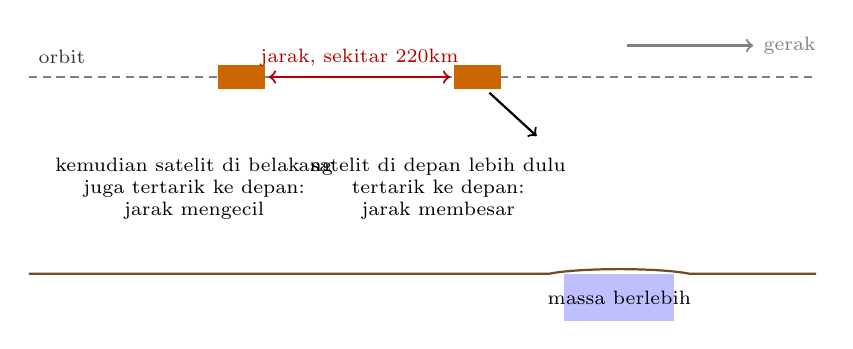
\begin{tikzpicture}[font=\small, x=1cm, y=1cm]
\draw[thick, brown!60!black] (-5,0) -- (1.6,0) .. controls (2.0,0.08) and (3.0,0.08) .. (3.4,0) -- (5,0);
\fill[blue!25] (1.8,0) rectangle (3.2,-0.6);
\node[font=\scriptsize] at (2.5,-0.3) {massa berlebih};
\draw[gray, densely dashed] (-5,2.5) -- (5,2.5);
\node[gray!40!black, font=\scriptsize, anchor=south west] at (-5,2.55) {orbit};
\fill[orange!80!black] (-2.6,2.35) rectangle (-2.0,2.65);
\fill[orange!80!black] (0.4,2.35) rectangle (1.0,2.65);
\draw[<->, red!70!black, thick] (-1.95,2.5) -- (0.35,2.5) node[midway, above, font=\scriptsize] {jarak, sekitar \qty{220}{km}};
\draw[->, thick] (0.85,2.3) -- (1.45,1.75);
\draw[->, thick, gray] (2.6,2.9) -- (4.2,2.9) node[right, font=\scriptsize] {gerak};
\node[font=\scriptsize, anchor=north, align=center] at (0.2,1.6) {satelit di depan lebih dulu\\tertarik ke depan:\\jarak membesar};
\node[font=\scriptsize, anchor=north, align=center] at (-2.9,1.6) {kemudian satelit di belakang\\juga tertarik ke depan:\\jarak mengecil};
\end{tikzpicture}

\par\smallskip{\small Prinsip pasangan satelit (skematis, tidak dalam
skala). Mendekati massa berlebih, satelit di depan merasakan tariknya
lebih dulu dan dipercepat ke depan, sehingga jarak di antara keduanya membesar; ketika
satelit di belakang melintasi massa itu, jarak kembali mengecil. Laju
jarak, yang diukur terus-menerus, diinversi untuk medan gravitasi.}
\label{fig:b3:gravity-geodesy:grace}
\end{omfigure}

\begin{omfigure}
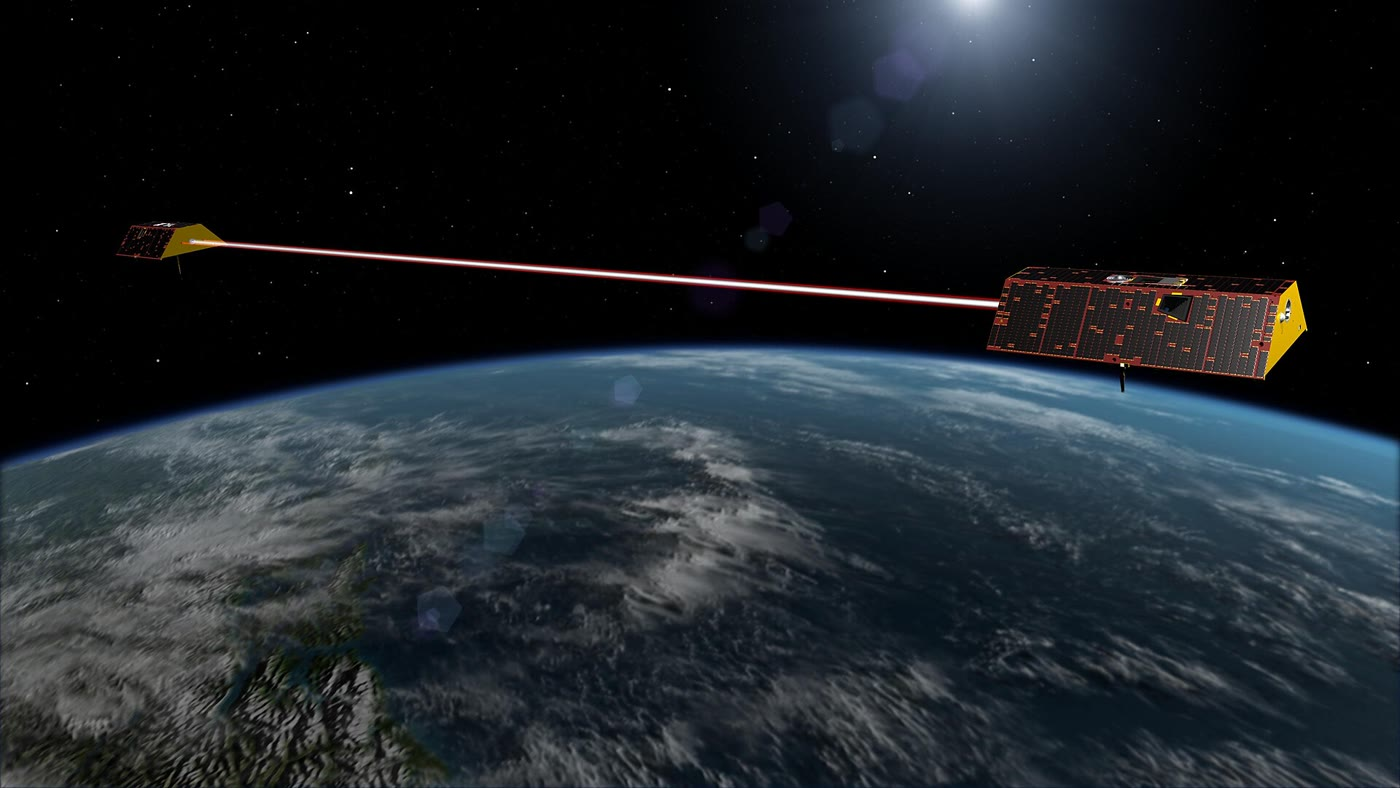
\includegraphics[width=0.66\linewidth]{images/book5/b3-grace-fo-concept.jpg}

\par\smallskip{\small Dua satelit GRACE Follow-On, gambaran artistik (jarak
di antara keduanya sangat diperpendek). Sinar merah mewakili tautan laser
pengukur jarak. NASA/JPL-Caltech, domain publik.}
\label{fig:b3:gravity-geodesy:grace-photo}
\end{omfigure}

\begin{definition}[Tinggi air setara]\label{def:b3:gravity-geodesy:ewh}
Perubahan medan gravitasi yang bervariasi lambat pada jarak jauh lebih besar
daripada ketebalan lapisan tempat massa berpindah dapat dinyatakan sebagai
perubahan rapat massa permukaan $\sigma$ (\unit{kg.m^{-2}}) pada kulit tipis di
permukaan Bumi. Yang disebut \emph{tinggi air setara}\index{tinggi air setara}
adalah ketebalan air tawar dengan rapat massa permukaan yang sama:
\[
  h_w = \frac{\sigma}{\rho_w} .
\]
\end{definition}

Satu meter air di atas cekungan seluas \qty{1e6}{km^2} sama dengan \qty{1e15}{kg}, atau
\qty{1000}{Gt}. Permukaan laut adalah sisi lain dari pembukuan ini: \qty{360}{Gt} es
yang ditambahkan ke samudra menaikkannya sekitar satu milimeter.
% ledger: data:b5-imbie
\omterm{def:b3:gravity-geodesy:satgrav}{Gravimetri satelit}, altimetri satelit, dan keseimbangan curah salju terhadap
pelepasan es masing-masing mengukur keseimbangan massa lembaran es; setelah digabungkan,
ketiganya memberikan deret di bawah ini.

\begin{omfigure}
\begin{tikzpicture}
\begin{axis}[omrecord, width=0.82\linewidth, height=0.5\linewidth,
  xmin=1992, xmax=2021, ymin=-5600, ymax=600,
  xlabel={tahun}, ylabel={perubahan massa kumulatif (\unit{Gt})},
  xticklabel style={/pgf/number format/1000 sep={}},
  legend pos=south west, legend cell align=left, legend style={font=\scriptsize}]
\addplot[name path=gl, draw=none, forget plot] table[x=year, y=lo] {figdata/out/bachelor-3-ice_mass-greenland.dat};
\addplot[name path=gh, draw=none, forget plot] table[x=year, y=hi] {figdata/out/bachelor-3-ice_mass-greenland.dat};
\addplot[blue!25, forget plot] fill between[of=gl and gh];
\addplot[name path=al, draw=none, forget plot] table[x=year, y=lo] {figdata/out/bachelor-3-ice_mass-antarctica.dat};
\addplot[name path=ah, draw=none, forget plot] table[x=year, y=hi] {figdata/out/bachelor-3-ice_mass-antarctica.dat};
\addplot[red!20, forget plot] fill between[of=al and ah];
\addplot[blue!70!black, thick] table[x=year, y=cum] {figdata/out/bachelor-3-ice_mass-greenland.dat};
\addlegendentry{Greenland}
\addplot[red!70!black, thick] table[x=year, y=cum] {figdata/out/bachelor-3-ice_mass-antarctica.dat};
\addlegendentry{Antarktika}
\draw[gray, densely dotted] (axis cs:2002.25,-5600) -- (axis cs:2002.25,600);
\draw[gray, densely dotted] (axis cs:2017.5,-5600) -- (axis cs:2017.5,600);
\node[font=\scriptsize, gray!40!black, anchor=north] at (axis cs:2009.9,550) {tahun GRACE};
\end{axis}
\end{tikzpicture}

\par\smallskip{\small Perubahan massa kumulatif lembaran es Greenland dan Antarktika
sejak 1992, dengan pita satu simpangan baku (taksiran IMBIE 2021 yang direkonsiliasi
dari altimetri, gravimetri, dan metode input--output). Pada akhir
2020 Greenland kehilangan $\num{4890} \pm \qty{460}{Gt}$ dan Antarktika
$\num{2670} \pm \qty{530}{Gt}$; kecocokan garis lurus memberikan
\qty{-176}{Gt.yr^{-1}} dan \qty{-91}{Gt.yr^{-1}} selama 1992--2020, dan
\qty{-246}{Gt.yr^{-1}} dan \qty{-127}{Gt.yr^{-1}} selama tahun GRACE.}
\label{fig:b3:gravity-geodesy:ice-mass}
\end{omfigure}

Anomali gravitasi yang diukur di permukaan adalah jumlah harmonik; pada
ketinggian satelit, masing-masing melemah oleh faktor yang bergantung pada
panjang gelombangnya.

\begin{proposition}[Kontinuasi ke atas]\label{prop:b3:gravity-geodesy:upward}
Di atas massa penyebabnya, anomali gravitasi yang bervariasi sepanjang permukaan
sebagai $\Delta g_0\cos kx$, dengan $k = 2\pi/\lambda$, pada ketinggian $z$ (\emph{kontinuasi
ke atas}\index{kontinuasi ke atas}) adalah
\[
  \Delta g(x, z) = \Delta g_0\,e^{-kz}\cos kx .
\]
\end{proposition}

\begin{proof}
Di atas massa, potensial anomali, dan bersama itu anomalinya, memenuhi
persamaan Laplace $\partial_x^2\Delta g + \partial_z^2\Delta g = 0$. Dengan memisahkan
peubah, $\Delta g = Z(z)\cos kx$ dengan $Z'' = k^2Z$, yang solusinya terbatas saat
$z \to \infty$ adalah $Z = \Delta g_0e^{-kz}$.
\end{proof}

Pada ketinggian \qty{400}{km}, anomali sepanjang \qty{1000}{km} mempertahankan \qty{8}{\percent}
dari amplitudonya, sedangkan yang sepanjang \qty{100}{km} tinggal sekitar \num{1e-11} darinya:
satelit mengamati gelombang panjang, dan survei di permukaan mengamati gelombang pendek.

\section{Lenturan litosfer}

Volume Tahun 1 mengompensasi beban secara lokal, tiap kolom mengapung sendiri.
Gunung api pada lempeng samudra tidak terkompensasi hanya di bawah dirinya sendiri: lempeng
melengkung di bawahnya pada lebar ratusan kilometer, dan dasar laut
di sekitar gunung api melesak membentuk parit, dan di luarnya ia naik membentuk lengkung rendah.

\begin{definition}[Lenturan litosfer, kekakuan lentur, ketebalan elastis efektif]\label{def:b3:gravity-geodesy:flexure}
Yang disebut \emph{lenturan litosfer}\index{lenturan litosfer} ialah pelengkungan
litosfer di bawah beban, dimodelkan sebagai lenturan lempeng elastis tipis
yang mengapung di atas mantel cair. Ketahanan lempeng terhadap pelengkungan ialah
\emph{kekakuan lentur}\index{kekakuan lentur}
\[
  D = \frac{ET_e^3}{12(1 - \nu^2)},
\]
dan ketebalan $T_e$ lempeng elastis seragam yang melentur seperti
litosfer sebenarnya ialah \emph{ketebalan elastis efektif}\index{ketebalan elastis efektif}.
\end{definition}

\begin{theorem}[Lenturan lempeng tipis]\label{thm:b3:gravity-geodesy:plate}
Lempeng elastis tipis dengan kekakuan $D$, dilentur sepanjang satu arah oleh beban $q(x)$
per satuan luas, melentur ke bawah sejauh $w(x)$ dan mengapung di atas mantel bermassa jenis
$\rho_m$, dengan cekungan terisi bahan bermassa jenis $\rho_i$, memenuhi
\emph{persamaan lenturan}\index{persamaan lenturan}
\[
  D\frac{\mathrm d^4w}{\mathrm dx^4} + (\rho_m - \rho_i)g\,w = q(x) .
\]
\end{theorem}

\begin{proof}
Pada lempeng yang melentur, serat di atas bidang tengah memendek dan serat di bawahnya
memanjang, sebanding dengan kelengkungan $w''$; mengintegralkan tegangan lentur
sepanjang ketebalan memberikan momen lentur $M = -Dw''$, dengan
kekakuan pada definisi (lempeng tidak dapat memuai ke samping, karena itu faktor
$1 - \nu^2$; volume Tahun 3 buku fisika). Sebuah irisan $\mathrm dx$ dari lempeng
memikul gaya geser $V$ pada kedua sisinya dan momen $M$. Keseimbangan vertikal:
beban $q\,\mathrm dx$ ke bawah dan daya apung mantel yang dipindahkan
$(\rho_m - \rho_i)gw\,\mathrm dx$ ke atas memberikan $\mathrm dV/\mathrm dx = -q +
(\rho_m - \rho_i)gw$. Keseimbangan momen memberikan $\mathrm dM/\mathrm dx = V$.
Maka $-Dw'''' = M'' = V' = -q + (\rho_m - \rho_i)gw$.
\end{proof}

\begin{definition}[Parameter lentur, tonjolan depan]\label{def:b3:gravity-geodesy:alpha}
Yang disebut \emph{parameter lentur}\index{parameter lentur} suatu lempeng ialah
panjang
\[
  \alpha = \left(\frac{4D}{(\rho_m - \rho_i)g}\right)^{1/4},
\]
yang menentukan skala horizontal lenturannya. Yang disebut \emph{tonjolan depan}\index{tonjolan depan}
ialah lengkungan rendah lenturan ke atas yang dibentuk lempeng melentur di luar parit atau
cekungan di sebelah bebannya.
\end{definition}

\begin{proposition}[Beban garis pada lempeng kontinu]\label{prop:b3:gravity-geodesy:line}
Beban garis $V_0$ per satuan panjang sepanjang $x = 0$ melenturkan lempeng sebesar
\[
  w(x) = w_0e^{-|x|/\alpha}\left(\cos\frac{|x|}{\alpha} + \sin\frac{|x|}{\alpha}\right),
  \qquad w_0 = \frac{V_0\alpha^3}{8D} .
\]
Lenturan menjadi nol pada $|x| = 3\pi\alpha/4$, tepi parit; puncak \omterm{def:b3:gravity-geodesy:alpha}{tonjolan depan}
berada di $|x| = \pi\alpha$, dengan tinggi $w_0e^{-\pi} =
\num{0.0432}\,w_0$. Daya apung seluruh lenturan menyeimbangkan beban:
$\int(\rho_m - \rho_i)gw\,\mathrm dx = V_0$.
\end{proposition}

\begin{proof}
Untuk $x > 0$ persamaannya ialah $w'''' + 4w/\alpha^4 = 0$; akar-akar dari
$r^4 = -4/\alpha^4$ adalah $(\pm1 \pm i)/\alpha$, dan solusi yang lenyap jauh
di sana ialah $e^{-x/\alpha}(A\cos(x/\alpha) + B\sin(x/\alpha))$. Simetri mensyaratkan
$w'(0) = 0$, yang memberikan $A = B = w_0$. Dengan mengintegralkan keseimbangan vertikal melintasi
beban, gaya geser $V = -Dw'''$ melompat sebesar $-V_0$; berdasarkan simetri
$w'''(0^-) = -w'''(0^+)$, dan $w'''(0^+) = 4w_0/\alpha^3$, sehingga $8Dw_0/\alpha^3 =
V_0$. Lenturan menjadi nol di mana $\tan(x/\alpha) =
-1$, pertama di $x = 3\pi\alpha/4$; turunannya,
$-(2w_0/\alpha)e^{-x/\alpha}\sin(x/\alpha)$, berikutnya menjadi nol di $x = \pi\alpha$.
Akhirnya $\int_0^\infty e^{-u}(\cos u + \sin u)\,\mathrm du = 1$, sehingga
$\int w\,\mathrm dx = 2w_0\alpha = V_0\alpha^4/(4D) = V_0/((\rho_m - \rho_i)g)$.
\end{proof}

\begin{proposition}[Lempeng patah]\label{prop:b3:gravity-geodesy:broken}
Lempeng yang patah di $x = 0$ dan didorong ke bawah pada ujung bebasnya, seperti pada
palung laut dalam, melentur sebagai $w = w_0e^{-x/\alpha}\cos(x/\alpha)$ untuk $x \ge 0$:
lenturan menjadi nol di $x = \pi\alpha/2$, dan puncak \omterm{def:b3:gravity-geodesy:alpha}{tonjolan depan}, yakni
kenaikan luar, berada di $x = 3\pi\alpha/4$, dengan tinggi $w_0e^{-3\pi/4}/\sqrt2 =
\num{0.067}\,w_0$.
\end{proposition}

\begin{proof}
\begingroup\emergencystretch=3em\relax Solusi peluruhan yang sama, kini dengan ujung bebas yang tidak memikul momen,
$w''(0) = 0$, yang memberikan $B = 0$. Nolnya berada pada $\cos(x/\alpha) = 0$;
turunannya $-(w_0/\alpha)e^{-x/\alpha}(\cos + \sin)(x/\alpha)$ lenyap pada
$x = 3\pi\alpha/4$, di mana $w = w_0e^{-3\pi/4}\cos(3\pi/4)$.
\par\endgroup\end{proof}

Jarak, dengan demikian, adalah kunci kekuatan lempeng: ukur di mana parit
berakhir atau di mana tonjolan mencapai puncak, dan $\alpha$ menyusul, lalu $D$, kemudian $T_e$.
Karena $T_e$ masuk sebagai $\alpha^{4/3}$, taksiran jarak yang wajar memberikan
taksiran ketebalan yang baik.

\begin{omfigure}
\begin{tikzpicture}
\begin{groupplot}[group style={group size=1 by 2, vertical sep=1.5cm},
  width=0.82\linewidth, height=0.36\linewidth, xmin=-400, xmax=400,
  tick label style={font=\scriptsize}, label style={font=\small}, title style={font=\small}]
\nextgroupplot[title={(a) Beban garis: punggungan Oru pada lempeng dengan tiga ketebalan},
  ylabel={lenturan (\unit{m})}, ymin=-3000, ymax=700, y filter/.expression={-y},
  legend pos=south east, legend cell align=left, legend style={font=\scriptsize}]
\addplot[red!70!black, thick] table[x=x, y=w10] {figdata/out/bachelor-3-flexure-profiles.dat};
\addlegendentry{$T_e = \qty{10}{km}$}
\addplot[blue!70!black, thick] table[x=x, y=w25] {figdata/out/bachelor-3-flexure-profiles.dat};
\addlegendentry{$T_e = \qty{25}{km}$}
\addplot[green!45!black, thick] table[x=x, y=w40] {figdata/out/bachelor-3-flexure-profiles.dat};
\addlegendentry{$T_e = \qty{40}{km}$}
\draw[gray] (axis cs:-400,0) -- (axis cs:400,0);
\draw[->, blue!70!black] (axis cs:222,330) -- (axis cs:222,90);
\node[font=\scriptsize, blue!70!black, anchor=south] at (axis cs:222,330) {tonjolan depan, $\pi\alpha$};
\nextgroupplot[title={(b) Lempeng patah di palung, $T_e = \qty{25}{km}$},
  xlabel={jarak dari beban atau palung (\unit{km})},
  ylabel={lenturan (\unit{m})}, xmin=0, xmax=400, ymin=-1100, ymax=280,
  y filter/.expression={-y}]
\addplot[blue!70!black, thick] table[x=x, y=w] {figdata/out/bachelor-3-flexure-broken.dat};
\draw[gray] (axis cs:0,0) -- (axis cs:400,0);
\draw[->] (axis cs:166.5,200) -- (axis cs:166.5,80);
\node[font=\scriptsize, anchor=west] at (axis cs:170,200) {kenaikan luar, $3\pi\alpha/4$};
\end{groupplot}
\end{tikzpicture}

\par\smallskip{\small Lenturan pelat elastis (dihitung;
$E = \qty{100}{GPa}$, $\nu = 0.25$, mantel \qty{3300}{kg.m^{-3}}, air di dalam
parit; skala vertikal sangat dilebih-lebihkan). (a) Di bawah beban gunung api
punggungan (\qty{4.17e12}{N.m^{-1}}), pelat tipis melesak dalam dan sempit, dan pelat
tebal melesak dangkal dan lebar; \omterm{def:b3:gravity-geodesy:alpha}{tonjolan depan} bergeser menjauh dari \qty{112}{km} ke
\qty{316}{km}. (b) Pelat yang patah di palung dan ditekan turun sejauh \qty{1}{km}:
kenaikan luar setinggi \qty{67}{m}, \qty{167}{km} dari palung.}
\label{fig:b3:gravity-geodesy:flexure}
\end{omfigure}

\begin{definition}[Kompensasi isostatik regional]\label{def:b3:gravity-geodesy:regional}
\emph{Kompensasi isostatik regional}\index{kompensasi isostatik regional}
adalah penopang beban oleh daya apung lenturan yang tersebar pada wilayah
yang lebih lebar daripada bebannya, melalui kekuatan lentur litosfer; pada kompensasi Airy
atau Pratt, sebaliknya, setiap kolom dikompensasi tepat di bawahnya sendiri.
\end{definition}

Kompensasi lokal dan regional menyeimbangkan massa total yang sama, tetapi mendistribusikannya
secara berbeda: di bawah beban sempit pada pelat kaku, akar lebih dangkal dan lebar,
dan anomali gravitasi di atas beban sangat positif, diapit anomali negatif
di atas parit. Di sekitar pulau-pulau Punggungan Hawaii, profil gravitasi dan
seismik memberikan \omterm{def:b3:gravity-geodesy:flexure}{ketebalan elastis efektif} 17 sampai \qty{37}{km}, dan
10 sampai \qty{20}{km} di sepanjang gunung laut tua pada rangkaian Emperor, selisih
yang diharapkan dari umur gunung api dan pelat yang mereka bebani; nilai-nilai
mengikuti kedalaman isoterm dekat
\qty{350}{\degreeCelsius} pada lempeng samudra yang mendingin.
% ledger: watts25:te
Lenturan yang sama, di bawah bobot sabuk pegunungan, membuka cekungan
depan-pegunungan pada volume Tahun 2, dalam babnya tentang orogenesis Alpen.

\begin{omfigure}
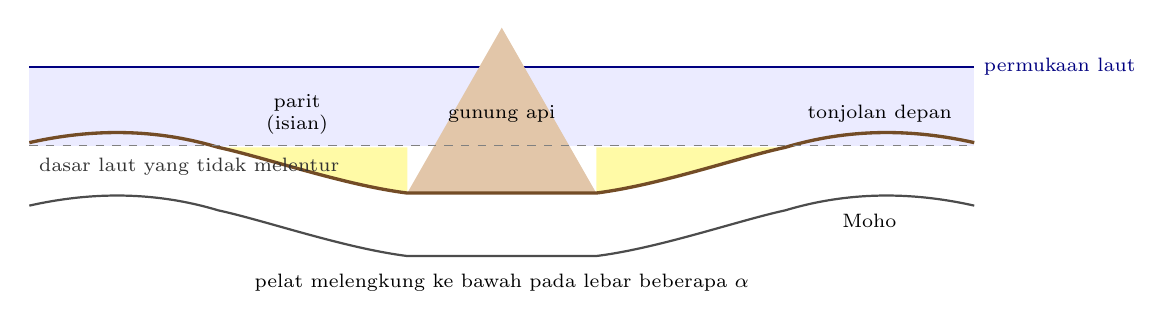
\begin{tikzpicture}[font=\scriptsize, x=1cm, y=1cm]
\fill[blue!8] (-6,0) rectangle (6,-1.0);
\draw[blue!50!black] (-6,0) -- (6,0) node[right] {permukaan laut};
% volcano
\fill[brown!45] (-1.2,-1.6) -- (0,0.5) -- (1.2,-1.6) -- cycle;
% moat infill
\fill[yellow!35] (-1.2,-1.6) .. controls (-2.0,-1.5) and (-3.0,-1.15) .. (-3.6,-1.02) -- (-1.2,-1.02) -- cycle;
\fill[yellow!35] (1.2,-1.6) .. controls (2.0,-1.5) and (3.0,-1.15) .. (3.6,-1.02) -- (1.2,-1.02) -- cycle;
% flexed seafloor (top of crust)
\draw[very thick, brown!60!black] (-6,-0.96) .. controls (-5.2,-0.78) and (-4.4,-0.78) .. (-3.6,-1.02)
  .. controls (-3.0,-1.15) and (-2.0,-1.5) .. (-1.2,-1.6) -- (1.2,-1.6)
  .. controls (2.0,-1.5) and (3.0,-1.15) .. (3.6,-1.02) .. controls (4.4,-0.78) and (5.2,-0.78) .. (6,-0.96);
% Moho, parallel
\draw[thick, gray!60!black] (-6,-1.76) .. controls (-5.2,-1.58) and (-4.4,-1.58) .. (-3.6,-1.82)
  .. controls (-3.0,-1.95) and (-2.0,-2.3) .. (-1.2,-2.4) -- (1.2,-2.4)
  .. controls (2.0,-2.3) and (3.0,-1.95) .. (3.6,-1.82) .. controls (4.4,-1.58) and (5.2,-1.58) .. (6,-1.76);
\node[anchor=west] at (4.2,-1.95) {Moho};
\draw[dashed, gray] (-6,-1.0) -- (6,-1.0);
\node[anchor=north west, gray!40!black] at (-6,-1.03) {dasar laut yang tidak melentur};
\node[anchor=south, align=center] at (-2.6,-0.98) {parit\\(isian)};
\node[anchor=south] at (4.8,-0.82) {tonjolan depan};
\node at (0,-0.6) {gunung api};
\node[anchor=north] at (0,-2.5) {pelat melengkung ke bawah pada lebar beberapa $\alpha$};
\end{tikzpicture}

\par\smallskip{\small Pulau gunung api di atas lempeng samudra (penampang skematik
melintang, skala vertikal dilebih-lebihkan). Pelat melengkung di bawah gunung api;
cekungan di sekelilingnya, yaitu parit, terisi puing gunung api dan sedimen, dan
di luarnya pelat naik membentuk \omterm{def:b3:gravity-geodesy:alpha}{tonjolan depan} yang rendah.}
\label{fig:b3:gravity-geodesy:moat}
\end{omfigure}

\begin{inthefield}[Survei gravitasi relatif]
\begin{minipage}[t]{0.55\linewidth}\vspace{0pt}
Gravimeter absolut menjatuhkan cermin sudut-kubus di dalam ruang hampa, berulang kali,
dan mengukur waktu jatuhnya dengan interferometer laser dan jam atom;
alat ini memberi gravitasi di satu stasiun, tetapi berat dan lambat dipasang. Survei
sendiri dilakukan dengan gravimeter relatif, yaitu neraca pegas kecil yang mengukur
selisih gravitasi. Geofisikawan menyeimbangkannya pada pelat dasar di setiap
stasiun sepanjang suatu lintasan, membacanya, mencatat waktu dan ketinggian, lalu berpindah; setiap
beberapa jam sekali lintasan kembali ke stasiun dasar, sehingga penyimpangan lambat
pegas dan pasang surut Bumi padat dapat diukur dan dihilangkan. Penerima satelit
di atas tiang di dekatnya memberikan posisi dan ketinggian, karena gravitasi
berubah sekitar \qty{0.3}{\milli\gal} untuk setiap meter ketinggian.
\end{minipage}\hfill
\begin{minipage}[t]{0.42\linewidth}\vspace{0pt}
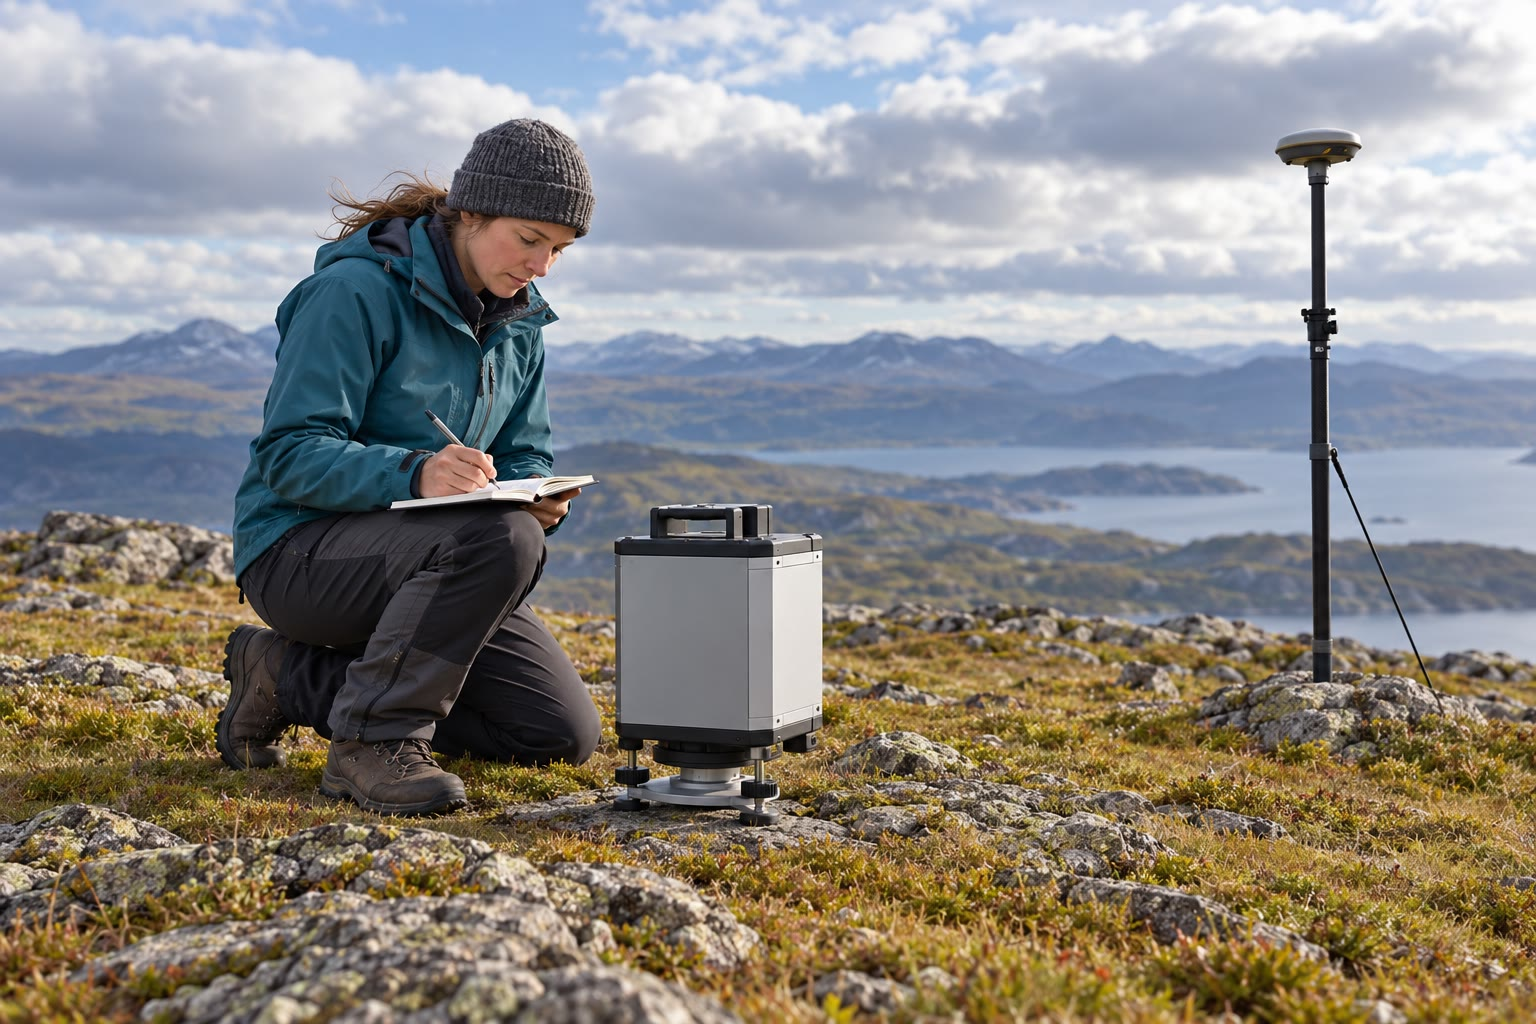
\includegraphics[width=\linewidth]{images/book5/ai/b3-gravimeter.jpg}

{\scriptsize Gravimeter lapangan di atas dasar penyeimbangnya, dengan antena satelit
di latar belakang (ilustrasi buatan AI).}
\end{minipage}
\end{inthefield}

\section{Latihan}

\begin{exercise}[$\star$]\label{exo:b3:gravity-geodesy:1}
Dari nilai Sistem Referensi Geodetik 1980 $a = \qty{6378137}{m}$ dan
$f = \num{0.00335281068}$, hitung sumbu semi-minor $b$ dan $a - b$. Dengan
$J_2 = \num{1.08263e-3}$ dan $m = \num{0.00344979}$, hitung penggepengan yang
diprediksi oleh hubungan Clairaut, lalu bandingkan.
\end{exercise}

\begin{exercise}[$\star$]\label{exo:b3:gravity-geodesy:2}
Pada tahun kering, cekungan sungai seluas \qty{5.0e5}{km^2} kehilangan \qty{60}{Gt}
air. Hitung perubahan \omterm{def:b3:gravity-geodesy:ewh}{tinggi air setara}. Seberapa besar massa yang sama akan
menaikkan permukaan laut, dengan \qty{360}{Gt} per milimeter?
\end{exercise}

\begin{exercise}[$\star$]\label{exo:b3:gravity-geodesy:3}
Dengan deret $\gamma = 9.780327(1 + 0.0053024\sin^2\varphi -
0.0000058\sin^22\varphi)$ \unit{m.s^{-2}}, hitung gravitasi normal di
khatulistiwa, pada \ang{45}, dan di kutub. Nyatakan selisih antara kutub
dan khatulistiwa dalam miligal.
\end{exercise}

\begin{exercise}[$\star$]\label{exo:b3:gravity-geodesy:4}
Hitung \omterm{def:b3:gravity-geodesy:flexure}{kekakuan lentur} dan \omterm{def:b3:gravity-geodesy:alpha}{parameter lentur} lempeng samudra dengan
$T_e = \qty{10}{km}$ dan $T_e = \qty{30}{km}$ ($E = \qty{100}{GPa}$,
$\nu = 0.25$, $\rho_m - \rho_w = \qty{2270}{kg.m^{-3}}$, $g =
\qty{9.81}{m.s^{-2}}$). Di mana letak tepi parit dan \omterm{def:b3:gravity-geodesy:alpha}{tonjolan depan} di bawah
beban garis?
\end{exercise}

\begin{exercise}[$\star\star$]\label{exo:b3:gravity-geodesy:5}
(a) Tinggi geoid sebesar $+\qty{50}{m}$: hitung potensial gangguan di sana,
dengan mengambil $\gamma = \qty{9.80}{m.s^{-2}}$. (b) Sepanjang \qty{100}{km}, geoid naik
sebesar \qty{10}{m}. Dengan sudut berapa garis unting-unting di situ menyimpang dari normal
terhadap elipsoid? Nyatakan dalam detik busur.
\end{exercise}

\begin{exercise}[$\star\star$]\label{exo:b3:gravity-geodesy:6}
Dari $J_2 = \num{1.08263e-3}$ dan faktor momen inersia
$C/(Ma^2) = \num{0.3308}$, hitung elipsitas dinamis $H = (C - A)/C$ dan
$1/H$. Di antara kedua bilangan itu, manakah yang akan berubah jika Bumi homogen dengan $J_2$ yang sama?
\end{exercise}

\begin{exercise}[$\star\star$]\label{exo:b3:gravity-geodesy:7}
Sebuah satelit bergerak pada orbit lingkaran \qty{500}{km} di atas jari-jari khatulistiwa
($a = \qty{6378.137}{km}$, $GM = \qty{3.986005e14}{m^3.s^{-2}}$), dengan kemiringan
\ang{89}. Hitung periodenya dan laju presesi simpul dalam derajat per hari.
Mengapa misi gravitasi memilih orbit dekat kutub?
\end{exercise}

\begin{exercise}[$\star\star$]\label{exo:b3:gravity-geodesy:8}
Dua anomali sebesar \qty{10}{\milli\gal} di permukaan memiliki panjang gelombang
\qty{100}{km} dan \qty{1000}{km}. Hitung amplitudo keduanya pada
ketinggian \qty{500}{km}.
\end{exercise}

\begin{exercise}[$\star\star$]\label{exo:b3:gravity-geodesy:9}
Di sisi laut parit, puncak tonjolan luar terletak \qty{120}{km} dari
sumbu parit. Dengan model lempeng patah dan air di atas lempeng, hitung
$\alpha$, $D$, dan $T_e$, serta jarak tempat lempeng memotong tingkat tanpa
lenturan.
\end{exercise}

\begin{exercise}[$\star\star\star$]\label{exo:b3:gravity-geodesy:10}
(a) Periksa bahwa $w = w_0e^{-u}(\cos u + \sin u)$, $u = x/\alpha$, memenuhi
$Dw'''' + (\rho_m - \rho_i)gw = 0$ untuk $x > 0$, dengan $\alpha$ seperti didefinisikan.
(b) Tunjukkan bahwa momen lentur $-Dw''$ paling besar di bawah beban dan berubah
tanda pada $x = \pi\alpha/4$. (c) Di mana lempeng paling mungkin retak di
permukaan atasnya, dan mengapa?
\end{exercise}

\begin{exercise}[$\star\star\star$]\label{exo:b3:gravity-geodesy:11}
Dengan $m = \num{0.00344979}$ dan $C/(Ma^2) = \num{0.3308}$, balikkan
hubungan Darwin--Radau untuk penggepengan hidrostatik. Bandingkan dengan
$f = \num{0.00335281}$: hitung selisihnya dan tinggi kelebihan khatulistiwa
di atas bentuk hidrostatik. Apa yang dikatakannya tentang mantel?
\end{exercise}

\begin{exercise}[$\star\star\star$]\label{exo:b3:gravity-geodesy:12}
Sebuah satelit pada orbit lingkaran setinggi \qty{700}{km} harus mempertahankan
orientasi yang sama terhadap Matahari sepanjang tahun: simpulnya harus maju \ang{360} dalam
satu tahun tropis \num{365.242}~hari. Hitung inklinasi yang diperlukan.
\end{exercise}

\section{Soal: Parit di sekitar punggungan Oru}

\begin{problem}[{Soal akhir pekan --- bentuk Bumi, beban vulkanik,
parit lenturnya dan apa yang dilihat satelit darinya}]
\label{pb:b3:gravity-geodesy:1}
% values: calc/ch03.py; GRS80 (geod5:grs80-*), earth:MoI; flexure.py
Oru adalah punggungan vulkanik rekaan di samudra: rangkaian lurus
gunung api yang menyatu sepanjang \qty{400}{km}, dibangun di atas litosfer samudra tua. Penampang melintangnya
diambil sebagai segitiga selebar \qty{80}{km} di alasnya dan
\qty{6}{km} tingginya, dengan massa jenis \qty{2800}{kg.m^{-3}}, berdiri di atas dasar laut
dengan kedalaman \qty{5}{km}. Mantel \qty{3300}{kg.m^{-3}}, air laut
\qty{1030}{kg.m^{-3}}, $E = \qty{100}{GPa}$, $\nu = 0.25$, $g =
\qty{9.81}{m.s^{-2}}$, $G = \qty{6.674e-11}{m^3.kg^{-1}.s^{-2}}$.

\medskip
\noindent\textbf{Bagian I --- Bentuk Bumi.} Gunakan Geodetic Reference
System 1980: $a = \qty{6378137}{m}$, $b = \qty{6356752.3}{m}$,
$GM = \qty{3.986005e14}{m^3.s^{-2}}$, $J_2 = \num{1.08263e-3}$,
$\omega = \qty{7.292115e-5}{rad.s^{-1}}$, $f = \num{0.00335281}$; dan
$C/(Ma^2) = \num{0.3308}$.
\begin{enumerate}
  \item Hitung $m = \omega^2a^2b/(GM)$.
  \item Hitung penggepengan yang diberikan hubungan Clairaut dari $J_2$ dan
        $m$, serta kebalikannya.
  \item Hitung penggepengan hidrostatik dari hubungan Darwin--Radau, serta
        kebalikannya.
  \item Bandingkan keduanya dengan penggepengan teramati. Berapa meter
        khatulistiwa berada di atas bentuk hidrostatik?
  \item Hitung elipsitas dinamis $H = (C - A)/C$.
\end{enumerate}

\noindent\textbf{Bagian II --- Beban.}
\begin{enumerate}[resume]
  \item Hitung luas penampang melintang punggungan.
  \item Hitung beban garis $V_0$, dengan menganggap seluruh punggungan terendam, sehingga
        beratnya $(\rho_v - \rho_w)g$ per satuan volume.
  \item Jika punggungan dikompensasi secara lokal, dengan cara Airy, oleh akar dari
        batuannya sendiri di dalam mantel, berapa dalam akar itu di bawah
        puncak?
  \item Dengan kompensasi lokal, akar itu akan berakhir di kaki punggungan,
        \qty{40}{km} dari sumbunya. Batimetri menunjukkan parit sampai
        \qty{165}{km}. Apa yang dapat kamu simpulkan dari hal ini?
\end{enumerate}

\noindent\textbf{Bagian III --- Parit lentur.} Parit itu terisi air
($\rho_i = \rho_w$). Profil seismik melintasi punggungan menemukan bagian atas
kerak samudra kembali ke kedalaman regionalnya \qty{165}{km} dari sumbu, dan
puncak \omterm{def:b3:gravity-geodesy:alpha}{tonjolan depan} \qty{220}{km} dari sumbu.
\begin{enumerate}[resume]
  \item Hitung \omterm{def:b3:gravity-geodesy:alpha}{parameter lentur} dari tepi parit.
  \item Hitung kembali dari \omterm{def:b3:gravity-geodesy:alpha}{tonjolan depan}. Apakah keduanya konsisten?
  \item Dengan $\alpha = \qty{70.0}{km}$, hitung \omterm{def:b3:gravity-geodesy:flexure}{kekakuan lentur}.
  \item Hitung \omterm{def:b3:gravity-geodesy:flexure}{ketebalan elastis efektif}.
  \item Dengan $V_0 = \qty{4.17e12}{N.m^{-1}}$ dan $D$ dibulatkan ke tiga
        angka penting, hitung defleksi di bawah sumbu.
  \item Hitung tinggi \omterm{def:b3:gravity-geodesy:alpha}{tonjolan depan}.
  \item Periksa bahwa daya apung seluruh defleksi, $2w_0\alpha(\rho_m -
        \rho_w)g$, mengimbangi $V_0$.
  \item Bandingkan $T_e$ dengan nilai yang diperoleh di sepanjang Punggungan Hawaii, 17 sampai
        \qty{37}{km}. Bandingkan defleksi di bawah sumbu dengan akar Airy
        pada pertanyaan 8.
\end{enumerate}

\noindent\textbf{Bagian IV --- Gravitasi di atas parit.} Ambil satu harmonik dari
lenturan, dengan panjang gelombang $2\pi\alpha$ dan amplitudo $W = \qty{500}{m}$, yang mendefleksikan
baik dasar laut (kerak \qty{2900}{kg.m^{-3}} di bawah air, \qty{5}{km} di bawah
permukaan laut) maupun Moho (mantel di bawah kerak, \qty{12}{km} di bawah permukaan laut). Sebuah
lapisan tipis dengan massa jenis permukaan $\sigma$ menghasilkan anomali $2\pi G\sigma$
tepat di atasnya.
\begin{enumerate}[resume]
  \item Hitung panjang gelombang dan bilangan gelombang $k$ dari harmonik itu.
  \item Hitung amplitudo anomali di permukaan laut akibat dasar laut yang
        terdefleksi, dikontinuasikan ke atas dari kedalaman \qty{5}{km}.
  \item Hitung amplitudo akibat Moho yang terdefleksi, serta totalnya.
  \item Hitung total pada ketinggian satelit, \qty{400}{km} di atas permukaan
        laut.
  \item Dengan faktor berapa harmonik dengan panjang gelombang \qty{80}{km}, lebar
        punggungan itu, melemah pada ketinggian tersebut? Apa yang dapat dibedakan satelit?
  \item Harmonik pada pertanyaan 18 sesuai dengan derajat harmonik bola $n \approx 2\pi R/\lambda$
        berapa ($R = \qty{6371}{km}$)?
  \item Berikan \omterm{def:b3:gravity-geodesy:flexure}{ketebalan elastis efektif} lempeng di bawah Punggungan
        Oru.
\end{enumerate}
\end{problem}
